% !TEX program = xelatex
% !BIB program = bibtex

\documentclass[UTF8]{article}

% layout
\usepackage[left=3cm,right=3cm]{geometry}
\usepackage{paralist} % for compactitem environment
\linespread{1.25}
% \makeatletter
% \def\@seccntformat#1{%
%   \expandafter\ifx\csname c@#1\endcsname\c@section
%   Section \thesection:
%   \else
%   \csname the#1\endcsname\quad
%   \fi}
% \makeatother
 
% page headings
\usepackage{fancyhdr}
\setlength{\headheight}{15.2pt}
\pagestyle{fancy}
\lhead{\leftmark}
\rhead{M201873026 Yilong Liu}
\cfoot{\thepage}
% \makeatletter
% \let\headauthor\@author
% \makeatother

% url/ref
\usepackage{hyperref}
\hypersetup{
  colorlinks,
  citecolor=black,
  filecolor=black,
  linkcolor=black,
  urlcolor=black,
  pdfauthor={Yilong Liu},
  pdftitle={Dataflow architecture: state-of-the-art and research challenges}
}

% vertical centering title page
\usepackage{titling}
\renewcommand\maketitlehooka{\null\mbox{}\vfill}
\renewcommand\maketitlehookd{\vfill\null}

% table of contents
\usepackage{tocloft}
\renewcommand\cftsecfont{\normalfont}
\renewcommand\cftsecpagefont{\normalfont}
\renewcommand{\cftsecleader}{\cftdotfill{\cftsecdotsep}}
\renewcommand\cftsecdotsep{\cftdot}
\renewcommand\cftsubsecdotsep{\cftdot}
\renewcommand{\contentsname}{\hfill\bfseries\Large Contents\hfill}   
\setlength{\cftbeforesecskip}{10pt}

% figures
\usepackage{graphicx}
\graphicspath{figures/}
% \newcommand\figureht{\dimexpr
%   \textheight-3\baselineskip-\parskip-.2em-
%   \abovecaptionskip-\belowcaptionskip\relax}

% tables
\usepackage{caption} 
\captionsetup[table]{skip=10pt}

% math, algorithms, code
\usepackage{amsmath,amssymb,url}
\usepackage{algorithm,algorithmicx,algpseudocode}
\usepackage{listings}

\lstset{
   extendedchars=true,
   basicstyle=\footnotesize\ttfamily,
   showstringspaces=false,
   showspaces=false,
   numbers=left,
   numberstyle=\footnotesize,
   numbersep=9pt,
   tabsize=2,
   breaklines=true,
   showtabs=false,
   captionpos=b
}

% bibliography
\usepackage[super,square,comma,sort]{natbib} % for \citet and \citep
\renewcommand{\refname}{References}
% \begin{filecontents}{report.bib}
% \end{filecontents} 

% appendix
\usepackage{appendix}

\title{Survey \\ \bigskip \textbf{Dataflow architecture: state-of-the-art and research challenges}}
\author{School of computer science and technology\\ M1801\\ M201873026\\ Yilong Liu}
\date{\today}

\begin{document}

\pagenumbering{gobble} % no page number
\maketitle
\newpage
% \null\thispagestyle{empty}
% \newpage

% \pagenumbering{roman}
% \section*{Abstract}\sectionmark{Abstract}
% \addcontentsline{toc}{section}{Abstract}
% \addcontentsline{toc}{section}{\protect\numberline{}Abstract}
% \newpage
% \pagenumbering{gobble} % no page number

\tableofcontents
\newpage
% \null\thispagestyle{empty}
% \newpage

\pagenumbering{arabic}

\section{Introduction}
Dataflow architecture is a computer architecture that
directly contrasts the traditional von Neumann architecture
or control flow architecture.
Dataflow architectures do not have a program counter,
or (at least conceptually) the executability
and execution of instructions is solely determined
based on the availability of input arguments to the instructions,
so that the order of instruction execution is unpredictable.
Dataflow architectures that are deterministic in nature
enable programmers to manage complex tasks
such as processor load balancing, synchronization and accesses to common resources.

The research, however, never overcame the problems related to:
\begin{compactitem}
  \item Efficiently broadcasting data tokens in a massively parallel system;
  \item Efficiently dispatching instruction tokens in a massively parallel system;
  \item Building CAMs large enough to hold all of the dependencies of a real program.
\end{compactitem}
Instructions and their data dependencies proved to be too fine-grained to be effectively distributed in a large network.
That is, the time for the instructions and tagged results to \textbf{travel} through a large connection network
was longer than the time to actually do the \textbf{computations}.

Designs that use conventional memory addresses as data dependency tags are called static dataflow machines.
These machines did not allow multiple instances of the same routines to be executed simultaneously
because the simple tags could not differentiate between them.
Designs that use content-addressable memory (CAM) or dynamic tagging are called dynamic dataflow machines.
They use tags in memory to facilitate \textbf{parallelism}.

\subsection{Computation Organization}
Mentioned in section~\ref{sec:dataflow_arch}.

Since a data-flow computer needs to record
the large set of potentially executable instructions,
it is difficult to conceive of supporting
data flow with a centralized machine organization.
Therefore proceed to support \textbf{packet communication}.

\subsection{Program Organization}

Programs are loaded into the CAM of a dynamic dataflow computer.
When all of the tagged operands of an instruction become available (that is, output from previous instructions and/or user input),
the instruction is marked as ready for execution by an execution unit.
This is known as activating or firing the instruction.
Once an instruction is completed by an execution unit,
its output data is sent (with its tag) to the CAM.
Any instructions that are dependent upon this particular datum (identified by its tag value)
are then marked as ready for execution.
In this way, subsequent instructions are executed in proper order, avoiding race conditions.
This order may differ from the sequential order envisioned by the human programmer, the programmed order.

An instruction, along with its required data operands,
is transmitted to an execution unit as a packet, also called an instruction token.
Similarly, output data is transmitted back to the CAM as a data token.
The packetization of instructions and results allows for parallel execution of ready instructions on a large scale.

The basic format of a reference (destination of data tokens) is $(P, N, A)$
and the fields are used for the following:
\begin{compactitem}
  \item The process (P) field distinguishes separate instances
        of an instruction N that may be executing in parallel,
        either within a single program or within distinct programs;
  \item The instruction (N) field identifies the consuming instruction
        to which the data token is being passed;
  \item The argument (A) field identifies in which
        argument position in the instruction N the token is to be stored. 
\end{compactitem}

\section{Dataflow Architecture}
\label{sec:dataflow_arch}
Survey of basic dataflow architecture.

Dennis~\cite{DBLP:conf/isca/DennisM74} proposed ``The Elementary Processor'',
as figure~\ref{fig:elementory_processor}.
When a Cell contains an instruction and the necessary operands,
it is enabled and signals the Arbitration Network
that it is ready to transmit its contents as an operationace
to an Operation Unit which can perform the desired function.
The result of an operation leaves an Operation Unit
as one or more data packet,
consisting of the computed value and the address of a register
in the Memory to which the value is to be delivered.
The Distribution Network accepts data packets
from the Operation Units and utilizes the address of each
to direct the data item through the network to the correct register in the Memory.
The Instruction Cell containing that register may then be enabled
if an instruction and all operands are present in the Cell.

\begin{figure}[htb]
  \begin{small}
    \begin{center}
      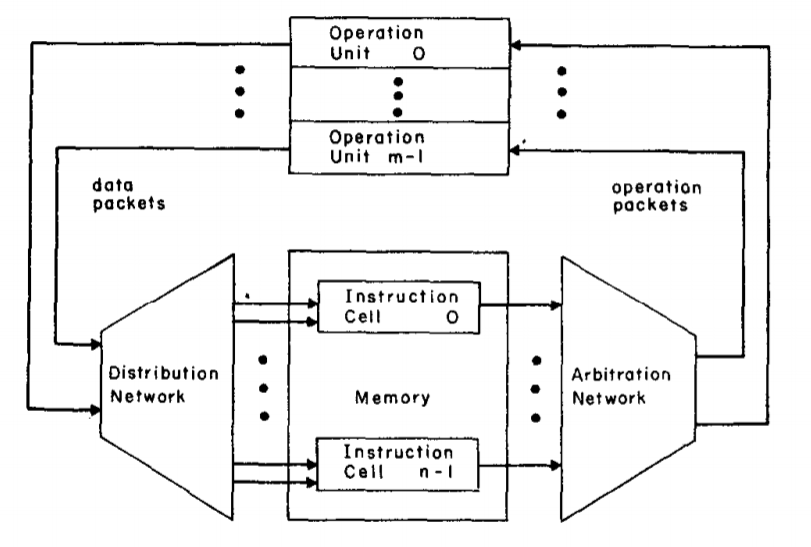
\includegraphics[width=\textwidth,height=8cm]{figures/isca94_elementory_processor.png}
    \end{center}
    \caption{ISCA94 - Elementary Processor.}
    \label{fig:elementory_processor}
  \end{small}
\end{figure}

Treleaven had a survey of dataflow architecture~\cite{DBLP:journals/csur/TreleavenBH82}.
Data flow is based on a by-value data mechanism
and a parallel control mechanism, supported by data tokens. 

The Manchester prototype dataflow computer~\cite{DBLP:journals/cacm/GurdKW85} proposed
a powerful dataflow processing engine based on dynamic tagging.
Instructions do not reference memory, since the data-dependence arcs
allow data to be transmitted directly from generating instruction to subsequent instruction.
Consequently, instructions can be viewed as \textbf{pure operations}.
Individual systems differ mainly in the way they handle re-entrant code.
Static systems do not permit concurrent reactivation,
and so they are restricted to implementing loops and cannot accommodate recursion.
Dynamic systems permit recursive reactivation,
either by code-copying or tagging, at every occurrence of re-entry.

The MIT tagged-token dataflow architecture~\cite{DBLP:journals/tc/ArvindN90} proposed
a novel multiprocessor dataflow architecture.
A traditional von Neumann processor has fundamental characteristics
that reduce its effectiveness in a parallel machine:
\begin{compactitem}
  \item its performance suffers in the presence of long memory and communication latencies;
  \item they do not provide good synchronization mechanisms
        for frequent task switching between parallel activities;
  \item it is a significant added complication for the programmer to manage parallelism explicitly.
\end{compactitem}
A token carries the address of an instruction in this fixed code,
and a dynamic context that specifies the frame for a particular invocation of the function.
The format of a token can now be seen: $(c, s, v)_p$.
Here, $c$ is the context, $s$ is the address of the destination instruction, $v$ is the datum,
and $p$ is the port identifying which input of the instruction this token is meant for.
The value $(c, s)$ is called the fag of the token.

TRIPS architecture~\cite{DBLP:conf/isca/SankaralingamNLKHBKM03} proposed

EDGE architecture~\cite{DBLP:journals/computer/BurgerKMDJLMBMY04} proposed

\clearpage

% \begin{table}
%   \begin{small}    
%     \caption{This is for long caption.}
%     \label{tab:table}
%     \begin{center}
%       \begin{tabular}[c]{l|l}
%         \hline
%         \multicolumn{1}{c|}{\textbf{xx}} & 
%         \multicolumn{1}{c}{\textbf{xx}} \\
%         \hline
% 	      a & b \\
% 	      c & d \\
% 	      e & f \\
%         \hline
%       \end{tabular}
%     \end{center}
%   \end{small}
% \end{table}

% \begin{algorithm}
%   \floatname{algorithm}{算法}
% 	\algrenewcommand\algorithmicrequire{\textbf{输入:}}
% 	\algrenewcommand\algorithmicensure{\textbf{输出:}}
% 	\caption{xxxxxxxxxx}
% 	\label{alg:main}
%   \begin{algorithmic}[1]
%     \State \textbf{return} $state$
% 	\end{algorithmic}  
% \end{algorithm}

% \begin{equation}
%   \text{UCT} = \frac{w_i}{s_i} + c\sqrt{\frac{\ln{s_p}}{s_i}}
%   \label{eq:uct}
% \end{equation}

\bibliographystyle{unsrt}
\bibliography{bibs/dataflow}
\addcontentsline{toc}{section}{References}
\newpage

\end{document}
